\documentclass[tikz,border=6pt]{standalone}
\usepackage{tikz}

\definecolor{paleyellow}{RGB}{255,239,160}
\definecolor{darkyellow}{RGB}{120,90,20}
\definecolor{midblue}{RGB}{120,170,225}
\definecolor{darkblue}{RGB}{20,50,130}
\definecolor{paleorange}{RGB}{255,205,150}
\definecolor{darkorange}{RGB}{160,75,15}

\tikzset{
  bigcell/.style={circle, draw=darkyellow, fill=paleyellow, text=darkyellow,
                  minimum size=8.8mm, font=\footnotesize\bfseries,
                  line width=0.4mm, inner sep=0pt},
  smallcell/.style={circle, draw=darkorange, fill=paleorange, text=darkorange,
                    minimum size=6mm, font=\tiny\bfseries,
                    line width=0.3mm, inner sep=0pt},
  chosencell/.style={circle, draw=darkblue, fill=darkblue, text=white,
                     minimum size=6mm, font=\tiny\bfseries,
                     line width=0.3mm, inner sep=0pt},
  dotnode/.style={circle, fill=black, minimum size=2.5mm, inner sep=0pt},
  pluslabel/.style={font=\footnotesize\bfseries}
}

\begin{document}
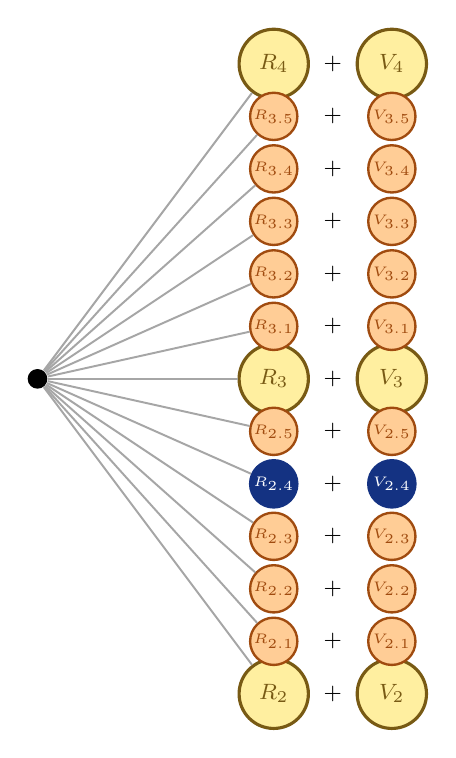
\begin{tikzpicture}[yscale=4]
  \node[dotnode] (p) at (-3, 3) {};

  \node[bigcell] (R2) at (0, 2) {$R_2$};
  \node[pluslabel] at (0.75, 2) {$+$};
  \node[bigcell] (V2) at (1.5, 2) {$V_2$};

  \node[bigcell] (R3) at (0, 3) {$R_3$};
  \node[pluslabel] at (0.75, 3) {$+$};
  \node[bigcell] (V3) at (1.5, 3) {$V_3$};

  \node[bigcell] (R4) at (0, 4) {$R_4$};
  \node[pluslabel] at (0.75, 4) {$+$};
  \node[bigcell] (V4) at (1.5, 4) {$V_4$};

  \foreach \k in {1,2,3,5} {
    \node[smallcell] (Rs2\k) at (0,   2 + \k/6) {$R_{2.\k}$};
    \node[pluslabel]         at (0.75, 2 + \k/6) {$+$};
    \node[smallcell] (Vs2\k) at (1.5, 2 + \k/6) {$V_{2.\k}$};
  }
  \node[chosencell] (Ropt) at (0,   2 + 4/6) {$R_{2.4}$};
  \node[pluslabel]         at (0.75, 2 + 4/6) {$+$};
  \node[chosencell] (Vopt) at (1.5, 2 + 4/6) {$V_{2.4}$};

  \foreach \k in {1,...,5} {
    \node[smallcell] (Rs3\k) at (0,   3 + \k/6) {$R_{3.\k}$};
    \node[pluslabel]         at (0.75, 3 + \k/6) {$+$};
    \node[smallcell] (Vs3\k) at (1.5, 3 + \k/6) {$V_{3.\k}$};
  }

  \draw[gray!70, line width=0.25mm] (p) -- (R2);
  \draw[gray!70, line width=0.25mm] (p) -- (R3);
  \draw[gray!70, line width=0.25mm] (p) -- (R4);
  \foreach \k in {1,2,3,5} {
    \draw[gray!70, line width=0.25mm] (p) -- (Rs2\k);
  }
  \draw[gray!70, line width=0.25mm] (p) -- (Ropt);
  \foreach \k in {1,...,5} {
    \draw[gray!70, line width=0.25mm] (p) -- (Rs3\k);
  }
\end{tikzpicture}
\end{document}
